\xchapter{Revisão da Literatura}{}
\label{revisao-lit}
Este capítulo aborda os principais fundamentos teóricos envolvidos na notificação oportuna de motoristas,
tema central deste trabalho, e traz uma revisão dos trabalhos relacionados com o tema. As seções deste capítulo
estão estruturadas da seguinte forma: A Seção \ref{interrupcao} apresenta os principais conceitos sobre interrupção
e seus efeitos sobre os motoristas. A Seção \ref{notificacao} fala sobre as notificações e seu efeito interruptivo.
A Seção \ref{contexto} discorre sobre contexto. Por fim, a Seção \ref{trabalhos-relacionados} apresenta os trabalhos
correlatos com o presente trabalho.

\section{Interrupção}
\label{interrupcao}
Controle cognitivo é o processo que permite que o comportamento do indivíduo e seu processamento de informação variem de momento a
momento, ao invés de se manterem rígidos e inflexíveis. O controle cognitivo pode ser expresso de várias maneiras, uma das quais
envolve a seleção do próximo pensamento para se focar, quando há múltiplas opções e quando distrações podem intervir.

Um exemplo do fato acima é uma conversação, que geralmente segue uma linha coerente. Se uma interrupção ocorre (um dos celulares dos
interlocutores começa a tocar, por exemplo) esta linha pode ser perdida, levando-os a se perguntar "Onde nós estávamos?" \cite{altmann2014momentary}.

Segundo \citeonline{ferreira2004novo}, interrupção é aquilo que faz parar uma ação ou um estado; o ato de cortar a continuidade de
algo. \citeonline{mcfarlane1997interruption} define interrupção humana como o processo de coordenar mudanças abruptas em uma atividade.

A interrupção durante a execução de uma tarefa pode ter vários efeitos adversos. \apudonline{lewin1927untersuchungen}{zijlstra1999temporal} diz
que pessoas lembram melhor dos detalhes de tarefas que não foram interrompidas. \citeonline{zijlstra1999temporal} concluem que
pessoas cometem mais erros em tarefas após uma interrupção. \citeonline{gillie1989makes} afirmam que as pessoas executam tarefas
mais vagarosamente após uma interrupção, se comparado com a performance pré-interrupção. Diante destas evidências, pode-se
afirmar que interrupções durante uma tarefa são bastante nocivas para a execução da mesma.

\subsection{Interrupção de Motoristas}
\label{interrupcao-motoristas}

Trabalhos anteriores estudaram os efeitos da execução de tarefas concorrentes com a direção. \citeonline{monk2004recovering} citam
que há diversos efeitos adversos ao executar tarefas cognitivas complexas durante a direção, como atraso na resposta a
acontecimentos repentinos, desatenção a informações sinalizadas, diminuição do controle do veículo, estreitamento do campo
de visão e mudanças de comportamento de frenagem e direção.

Além disso, vários problemas na execução de uma tarefa após uma interrupção, como os citados na Seção \ref{interrupcao}, afetam o
motorista durante a direção de um veículo:

\begin{itemize}
  \item Ao não lembrar de detalhes do que estava fazendo antes da interrupção, o motorista pode esquecer de informações
  apontadas pela sinalização de trânsito;
  \item Ao cometer erros após uma interrupção, o motorista põe em risco a si mesmo e a seus pares, podendo causar acidentes
  de trânsito;
  \item Ao reagir mais vagarosamente após uma interrupção, o motorista fica vulnerável a ameaças externas que exijam de sua
  capacidade reativa;
\end{itemize}

O estudo de \citeonline{monk2004recovering} ainda conclui que interrupções antes ou depois de uma tarefa ou sub-tarefa trazem
menos problemas, e cita curvas, mudanças de faixa e entrada em uma rodovia como exemplos de sub-tarefas que o motorista executa.
Este fato serve de justificativa para a escolha dos momentos inoportunos a serem detectados neste trabalho, que são a curva
e mudança de faixa.

Estima-se que o uso de celular durante o ato de dirigir um veículo aumenta o risco de acidentes em 38\% \cite{laberge2001wireless}.
Em paralelo a este fato, \citeonline{stothart2015attentional} afirmam que apenas o ato de receber uma notificação, mesmo que ela não seja
atendida, distrai o motorista tanto quanto receber uma ligação no celular ou responder uma mensagem de texto. Ante este fato, é
necessário estudar as notificações e sua capacidade de interromper tarefas.

\section{Notificações e seu caráter interruptivo}
\label{notificacao}

Notificação pode ser definida como um sinal visual, audível ou táctil, gerado por uma aplicação
ou serviço e que passa informação para um usuário que está fora de seu foco de atenção \cite{iqbal2010notifications}.
Em dispositivos móveis, notificações geralmente são enviadas instantaneamente no momento em que ocorre alguma atividade que pode ser relevante
para o usuário quando a aplicação não está aberta, ex: um email novo, uma mensagem de texto que acaba de chegar ou um
novo comentário em suas redes sociais. Em alguns casos o usuário toma ações imediatas após a chegada da notificação,
enquanto em outros ela é simplesmente ignorada. Essas ações dependem da importância da notificação e do contexto do
usuário \cite{sahami2014large}.

Em dispositivos móveis uma notificação é uma mensagem que pode ser exibida ao usuário fora da interface normal de um aplicativo.
Quando o aplicativo emite uma notificação, ela primeiro aparece como um ícone na área de notificação. No sistema operacional móvel
Android \cite{android}, para ver os detalhes da notificação, o usuário abre a gaveta de notificação \cite{notificationDrawer}. A Figura
\ref{notification-drawer} mostra o layout da gaveta de notificações no Android. Cada retângulo branco preenchido com ícones
e texto representa uma notificação diferente. O horário de chegada aparece no canto direito de cada notificação.

Notificações semelhantes geralmente são agrupadas para que não sejam exibidas inúmeras notificações com conteúdo parecido.
Pode-se perceber na Figura \ref{notification-drawer} que a maioria das notificações possui um indicativo de informações agrupadas
ao invés de múltiplas notificações. Ex: O texto "\textit{3 new messages}" que aponta que existem 3 novas mensagens, ao invés de 3
notificações apontando 1 nova mensagem cada.

A maioria das notificações possui pelo menos uma ação atrelada a si. Uma ação permite que os usuários passem
diretamente da notificação para uma tela específica do aplicativo, onde podem visualizar um ou mais eventos ou realizar
outros trabalhos.

\begin{figure}[h]
\centering
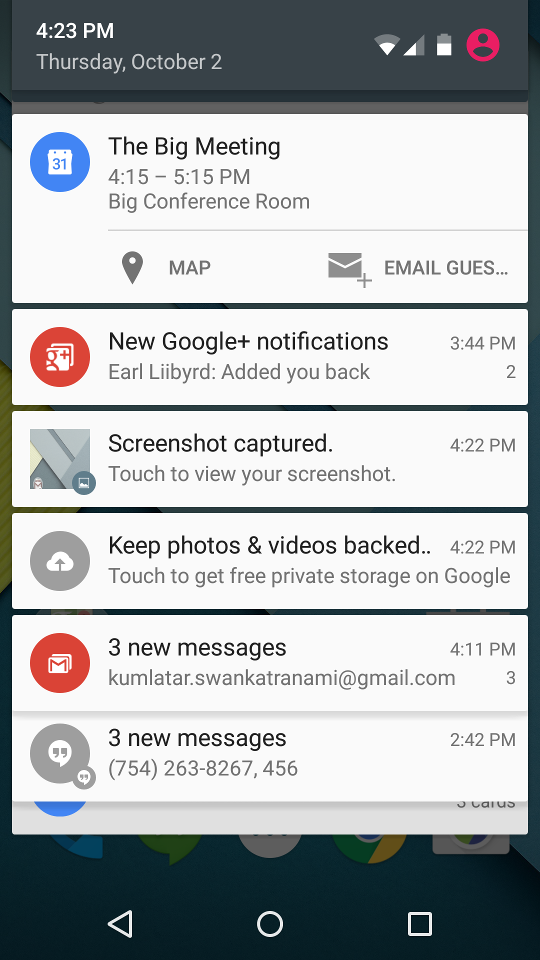
\includegraphics[width=0.3\textwidth]{images/notification_drawer.png}
\caption{Exemplo de notificações no Android \cite{notificationDrawer}}
\label{notification-drawer}
\end{figure}

A área de notificação e a gaveta de notificação mostradas na Figura \ref{notification-drawer} são áreas controladas pelo
sistema operacional e que o usuário pode visualizar a qualquer momento.

Cada vez que um dispositivo provê informação proativamente (ex: Notificando que há um novo comentário em suas redes
sociais) ele está competindo pela atenção do usuário e possívelmente interrompendo tarefas que estão acontecendo no momento
\cite{ho2005using}. Alguns estudos tentaram entender a relação dos usuários com este efeito adverso.

\citeonline{oulasvirta2012habits} discorrem sobre os hábitos de uso de smartphones. Os autores descobriram que o rápido acesso a
conteúdo dinâmico pode criar hábitos, que ficam mais fortes com o aumento da frequência de uso do dispositivo. Eles
também mencionam que estes hábitos são uma característica particular do uso de smartphones e que ainda não são percebidos
pela sociedade como problemáticos. \citeonline{iqbal2010notifications} concluem em seu estudo que usuários valorizam o sentimento
de informação que as notificações trazem e que, mesmo cientes de seus efeitos interruptivos, preferem manter este sentimento.

Estes achados permitem a conclusão que apesar de sua capacidade interruptiva, notificações são valorizadas pelos
usuários e fazem parte do próprio hábito de uso dos smartphones. Por este motivo, é necessário que se diminua o potencial
interruptivo das notificações, o que pode ser conseguido utilizando contexto, como sinalizam alguns autores
\cite{ho2005using, kern2003context, iqbal2010notifications}.

\section{Contexto}
\label{contexto}

Em 1991 é cunhado o termo "Computação Ubíqua", que se refere ao caráter invisível da integração de dispositivos
computacionais diversos e da adaptação dos mesmos à necessidade do usuário no momento \cite{weiser1991computer}.
Um elemento bastante importante para a Computação Ubíqua é o estudo do contexto.

Contexto é definido por \citeonline{dey2001understanding} como "Qualquer informação que pode ser utilizada para
caracterizar a situação de entidades (ex: um usuário, lugar ou objeto) e que é considerada relevante para
a interação entre um usuário e uma aplicação, incluindo o próprio usuário e aplicação". Esta definição é
a mais utilizada na área. Alguns exemplos de elementos de contexto são
localização do usuário, identidade do usuário e tempo \cite{ryan1999enhanced}.

Diversos sensores podem ser utilizados para determinar informações sobre o contexto do usuário. Alguns exemplos são
sensores de localização (GPS - \textit{Global Positioning System}, em português Sistema de Posicionamento Global),
sensores de luz, acelerômetro e giroscópio.

Informações de contexto são importantes para definir o estado atual do usuário e do ambiente onde ele está inserido,
mas somente isto é insuficiente. Para utilizar estas informações satisfatoriamente é ideal que se construa um sistema
adaptativo e que supra as necessidades do usuário em tempo real utilizando as informações de contexto. Resumindo,
um sistema sensível ao contexto.

Sistemas sensíveis ao contexto são capazes de adaptar suas operações ao contexto atual, sem intervenção
explícita do usuário e têm como objetivo aumentar sua usabilidade e efetividade levando em conta elementos
de contexto \cite{baldauf2007survey}.  Um sistema é sensível ao contexto se ele utiliza contexto para prover
informações relevantes e/ou serviços para usuários, sendo que a relevância depende das tarefas do usuário
\cite{abowd1999towards}.

Este trabalho propõe a construção de um sistema sensível ao contexto que identifica momentos oportunos e inoportunos para
o envio de notificações a motoristas, utilizando apenas sensores de um smartphone comum.

\section{Trabalhos Relacionados}
\label{trabalhos-relacionados}

Em pesquisas preliminares não encontramos nenhuma aplicação, solução ou proposta que construiu um sistema para
notificação de motoristas em momentos oportunos utilizando contexto. Entretanto, encontramos projetos de aplicações que
usam dados de contexto para detectar aspectos relacionados ao comportamento de motoristas.

\citeonline{kim2015sensors} desenvolveram um classificador utilizando aprendizagem de máquina para detectar a interruptibilidade
de motoristas em um dado momento. Para a coleta de dados foram utilizados um sensor fisiológico vestível, quatro sensores
de movimento também vestíveis, câmeras direcionadas ao tráfego e ao motorista e um dispositivo OBD (\textit{On-Board Diagnostic},
em português Sistema de Diagnóstico de Bordo), como mostrado na Figura \ref{kim-sensors}.

\begin{figure}[h]
\centering
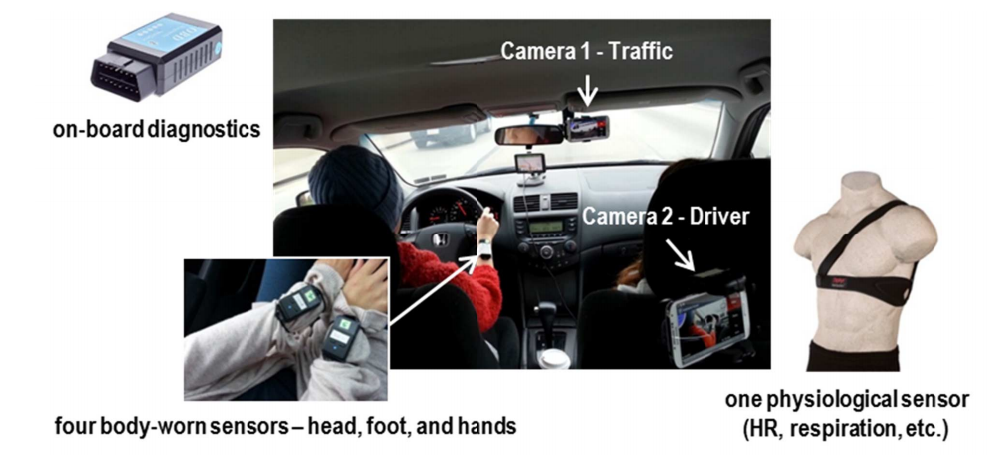
\includegraphics[width=0.9\textwidth]{images/kim-sensors.png}
\caption{Sensores utilizados no trabalho de \citeonline{kim2015sensors}.}
\label{kim-sensors}
\end{figure}

Um experimento foi feito com 25 motoristas (14 mulheres e 11 homens), com idade entre 19 e 69 anos, consistindo em 2 seções
onde os motoristas dirigiam de um ponto a outro. O resultado do experimento mostrou que interrupções têm menos impacto em um motorista
quando ele não está com nenhuma das mãos no volante ou quando está interagindo com um periférico (controlador do ar condicionado, por exemplo).
O classificador para detecção de interruptibilidade construído obteve 94\% de precisão na detecção de momentos
oportunos para interrupção de motoristas.

O trabalho de \citeonline{kim2015sensors} também apresenta evidências de que há outros momentos oportunos para interromper motoristas, como
por exemplo quando o carro está parado (todas as vezes em que o motorista não tinha nenhuma das mãos no volante, a velocidade do carro era menor
do que 3 km/h), quando a velocidade do carro é baixa e quando a velocidade é constante. Estes achados servem como justificativa para a
escolha dos momentos oportunos a serem detectados neste trabalho, que são o veículo parado e a velocidade baixa e constante.

%O presente trabalho visa construir um classificador semelhante, com o diferencial de utilizar apenas sensores de smartphone.

\citeonline{johnson2011driving} apresentam o MIROAD (sigla em inglês para Plataforma Móvel para Reconhecimento
Inteligente de Direção Agressiva), que é um sistema para detectar comportamentos agressivos durante a direção de um veículo, utilizando
apenas sensores de smartphone. Os sensores utilizados são a câmera traseira, acelerômetro, giroscópio e GPS. O setup utilizado para este
sistema está demonstrado na Figura \ref{miroad}.

\begin{figure}[h]
\centering
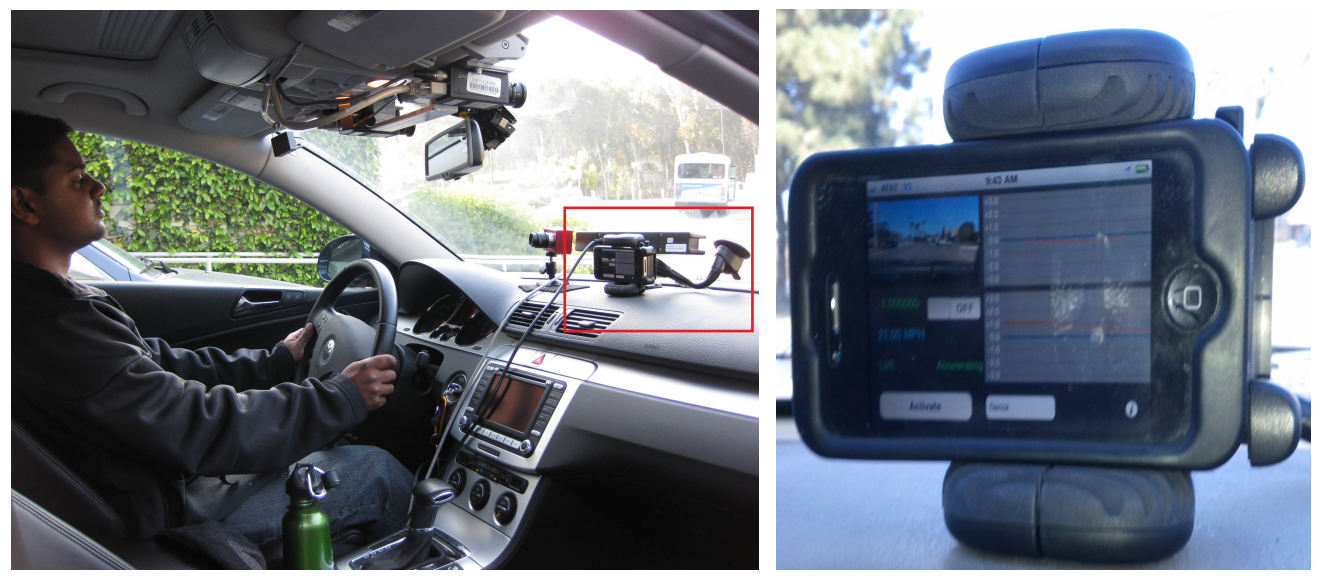
\includegraphics[width=0.7\textwidth]{images/miroad.png}
\caption{Sensores utilizados no MIROAD. \cite{johnson2011driving}}
\label{miroad}
\end{figure}

O MIROAD coleta dados continuamente do acelerômetro e giroscópio para detectar algumas manobras específicas, como curvas acentuadas
e acelerações e freadas instantâneas.
Um experimento foi feito e obteve cerca de 97\% de corretude. Estes resultados demonstram que é possível construir
um mecanismo para predição de comportamento veicular utilizando apenas sensores do smartphone e contribuem para a motivação deste trabalho.

\citeonline{eren2012estimating} apresentam um trabalho semelhante que tenta estimar o comportamento na direção de motoristas como seguro ou
não seguro, utilizando algoritmo de detecção de melhor caminho e classificação Bayesiana. Este sistema utiliza
apenas sensores de smartphone (acelerômetro, giroscópio e magnetômetro) para adquirir dados de contexto e obteve
resultados corretos em 14 casos de 15.

\citeonline{park2016integrated} desenvolveram um sistema integrado com direção veicular chamado de IDAS para conduzir estudos de experiência
do usuário (UX). Este sistema coleta dados do motorista e do veículo, analiza-os e provê um feedback visual baseado
nas informações que o motorista precisa no momento. São utilizados sensores vestíveis para aquisição de dados
fisiológicos e de movimentação do motorista, um dispositivo OBD para obtenção de dados veiculares, um GPS veicular e as informações
são exibidas em um aplicativo Android. O setup utilizado é mostrado na Figura \ref{idas}.

\begin{figure}[htb]
\centering
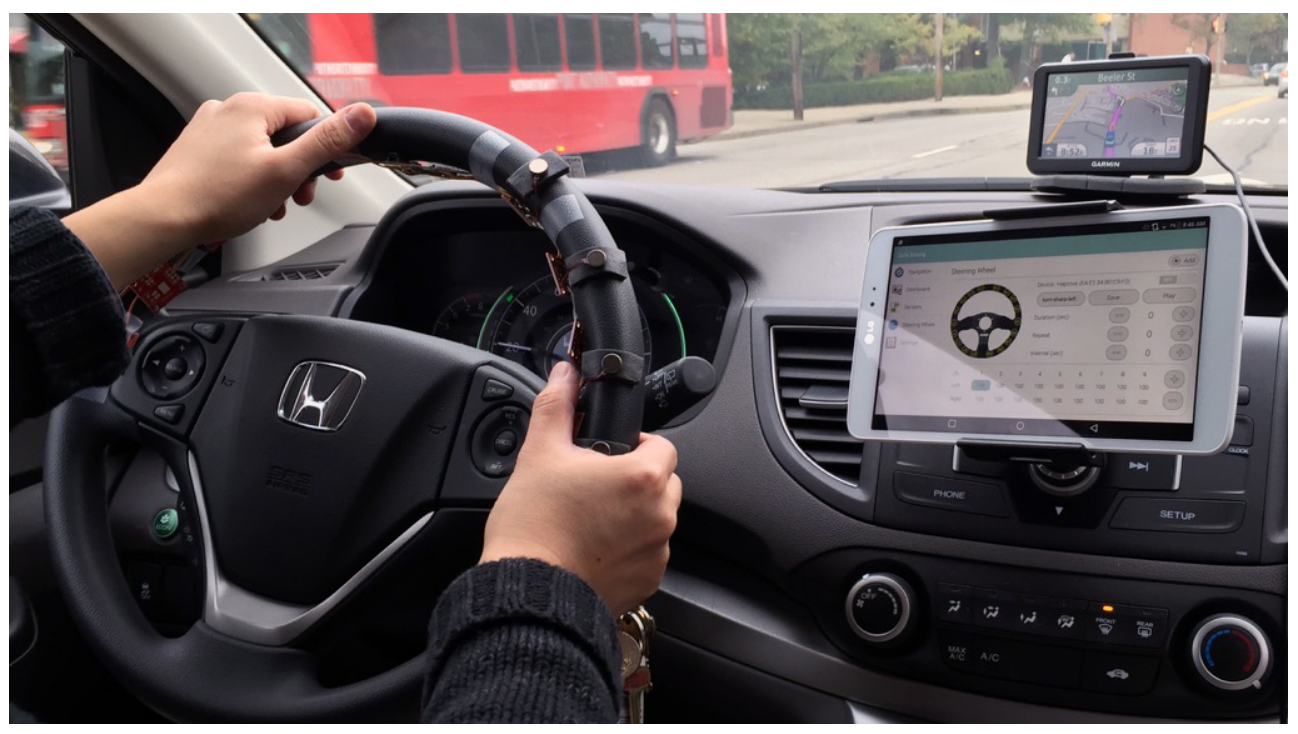
\includegraphics[width=0.7\textwidth]{images/idas.png}
\caption{Sensores utilizados no IDAS. \cite{park2016integrated}}
\label{idas}
\end{figure}

Trabalhos anteriores também corroboram a tese de que é possível utilizar sensores para prever a interruptibilidade
humana em um dado momento. \citeonline{fogarty2005predicting} construíram um modelo que utiliza sensores de áudio e vídeo
para estimar a interruptibilidade de trabalhadores de escritório em um dado momento. \citeonline{hudson2003predicting}
construíram um modelo semelhante utilizando os mesmos sensores e obtiveram uma média de 75\% de acurácia na predição de
interruptibilidade de trabalhadores de escritório.

O presente trabalho propõe um sistema que identifica momentos oportunos e inoportunos para interrupção de motoristas.
Este sistema funcionará junto a um aplicativo pré-existente. O próximo capítulo apresenta mais detalhes sobre o referido
aplicativo e sobre a arquitetura e implementação da proposta.
